\section{Introdução}

Este relatório apresenta os resultados de testes geofísicos realizados para avaliar a densidade geológica em um determinado ambiente. Os testes foram realizados com base na densidade hiperbólica, que é uma técnica amplamente utilizada para estimar a densidade de rochas e minerais em subsuperfície. Para isso, foram realizados pelo menos dois testes distintos, variando os parâmetros do contraste de densidade e do fator de variação da densidade com a profundidade. As análises foram feitas com base nas curvas ajustadas e distantes da Figura~\ref{Figura 1}, que mostram as anomalias gravimétricas resultantes da estrutura geológica em subsuperfície. As imagens obtidas durante os testes também serão apresentadas para justificar as análises e interpretações dos resultados.

        \begin{figure}[!h]  
        \centering
        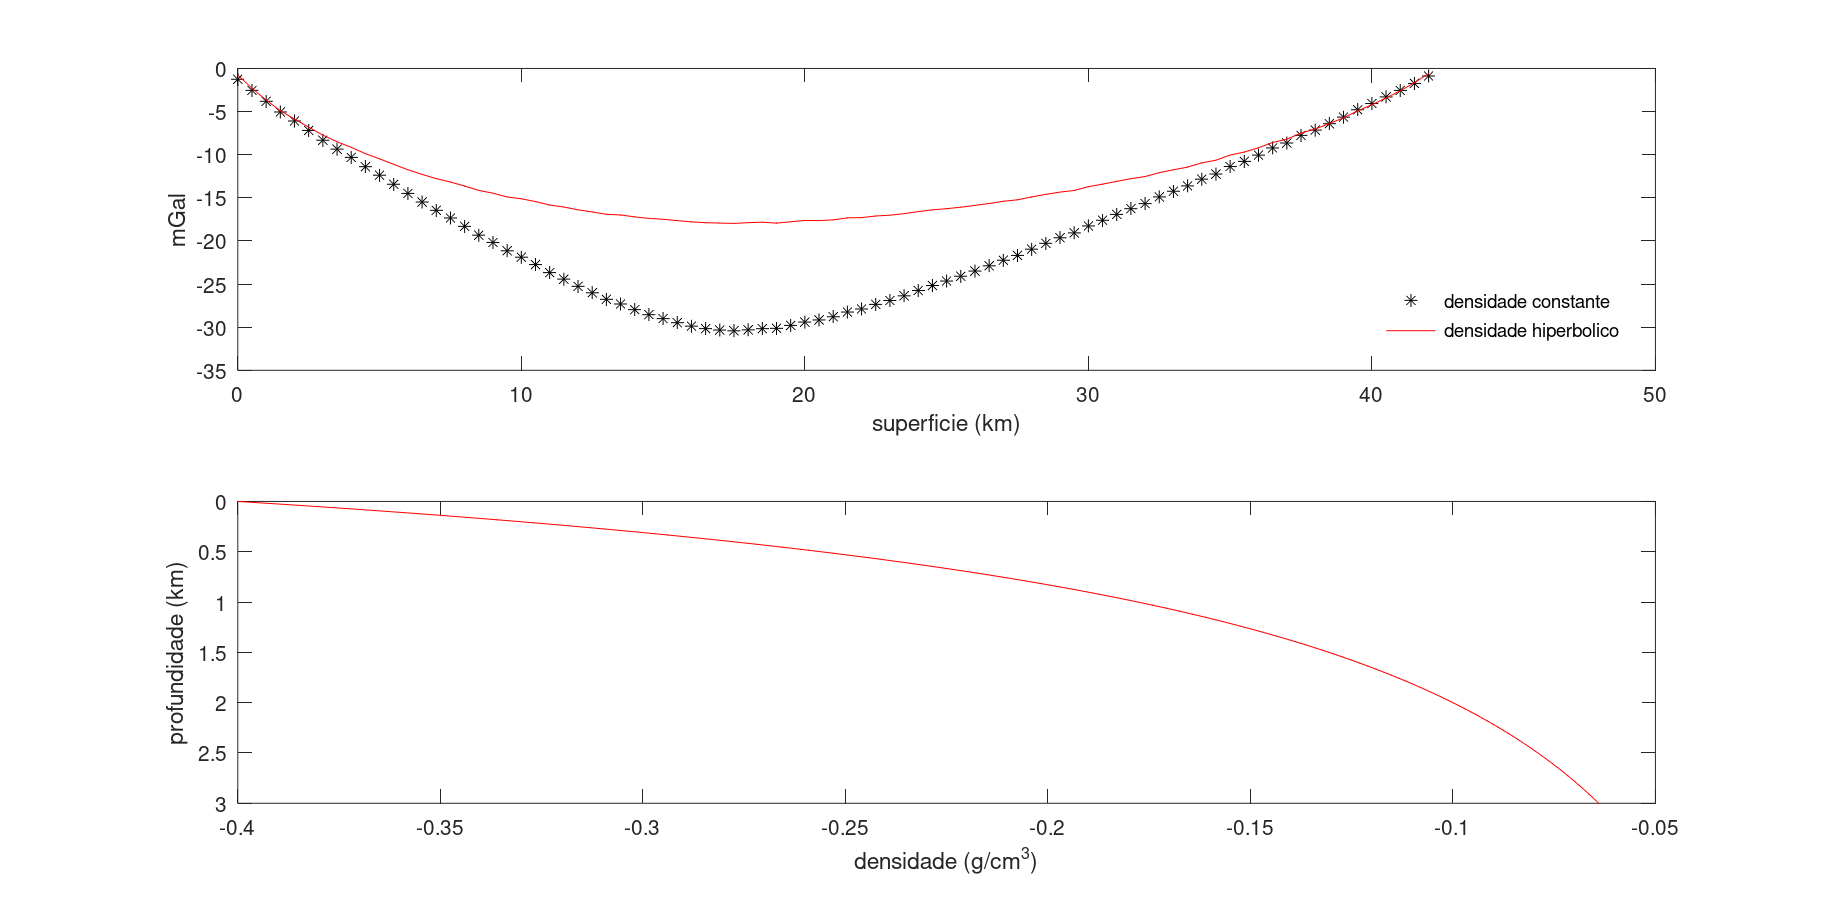
\includegraphics[height=8cm]{figure/Imagem inicial.png}
        \caption{Representação dos Parâmetros inicias, sem alterações(Leia-se a 1ª e 2ª imagem como: A e B).}
        \label{Figura 1}
        \end{figure}
        
A função hiperbólica é uma expressão matemática que pode ser usada para representar a variação da densidade dos sedimentos com a profundidade em bacias sedimentares. Ela foi introduzida por Litinsky em 1989 e, em certos casos, pode fornecer um ajuste melhor para dados de densidade/profundidade do que a função exponencial \cite{sari2002analysis}. Além disso, os modelos de gravidade de uma bacia requerem o uso de expressões com contraste de densidade hiperbólica em relação à anomalia produzida pelo modelo. A densidade dos sedimentos aumenta com a profundidade, principalmente devido à compactação, aproximando-se da densidade do embasamento em bacias profundas.
%\lipsum[1-3] % Remover

%\nocite{leithold, moyses, peruzzo} % Remova
